\documentclass[
    % handout,
    center,
    % aspectratio=169
]{beamer}

\usepackage[utf8]{inputenc}
\usepackage[english]{babel}
\usepackage{graphicx}
\usepackage{amsmath,amssymb,amsfonts}
\usepackage{booktabs}
\usepackage{tabularx}
\usepackage[ruled,vlined]{algorithm2e}

\graphicspath{../}

\title[Deep Learning Camera Pose Estimation]{\textsc{A Deep Learning Approach to\\Camera Pose Estimation}}
\author[Bozzo - Izzo]{Federico Izzo \and Francesco Bozzo}
\institute[UniTN]{University of Trento}
\date{January 12, 2022}

% \logo{\includegraphics[height=1.5cm]{logo.png}}
\usetheme{Madrid}
\definecolor{links}{HTML}{54489a}
\hypersetup{colorlinks,linkcolor=,urlcolor=links}
% \usetheme{metropolis} 


\begin{document}

\begin{frame}
    \titlepage
\end{frame}

% \AtBeginSection[]
% {
%     \begin{frame}{Table of Contents}
%         \begin{columns}[t]
%             \column{.45\textwidth}
%             \tableofcontents[sections=1-2, currentsection]

%             \column{.45\textwidth}
%             \tableofcontents[sections=3-5, currentsection]
%         \end{columns}
%     \end{frame}
% }

\section{Introduction}
\begin{frame}{Introduction}
    With this work we are going to present:
    \begin{itemize}
        \item the exploration of multiple dataset generation techniques;
        \item the COLMAP reconstruction of Povo 1 second floor;
        \item the development of relative and absolute pose estimation models;
        \item the fine-tuning of absolute pose estimation models;
        \item the post-processing of the model outputs;
        \item the model deployment using a FastAPI web-server. 
    \end{itemize}
\end{frame}

% what is camera pose estimation: introdution image (with formulas?)
\begin{frame}{Camera pose estimation}
    \begin{columns}
        \column{0.45\textwidth}
        \begin{figure}
            \centering
            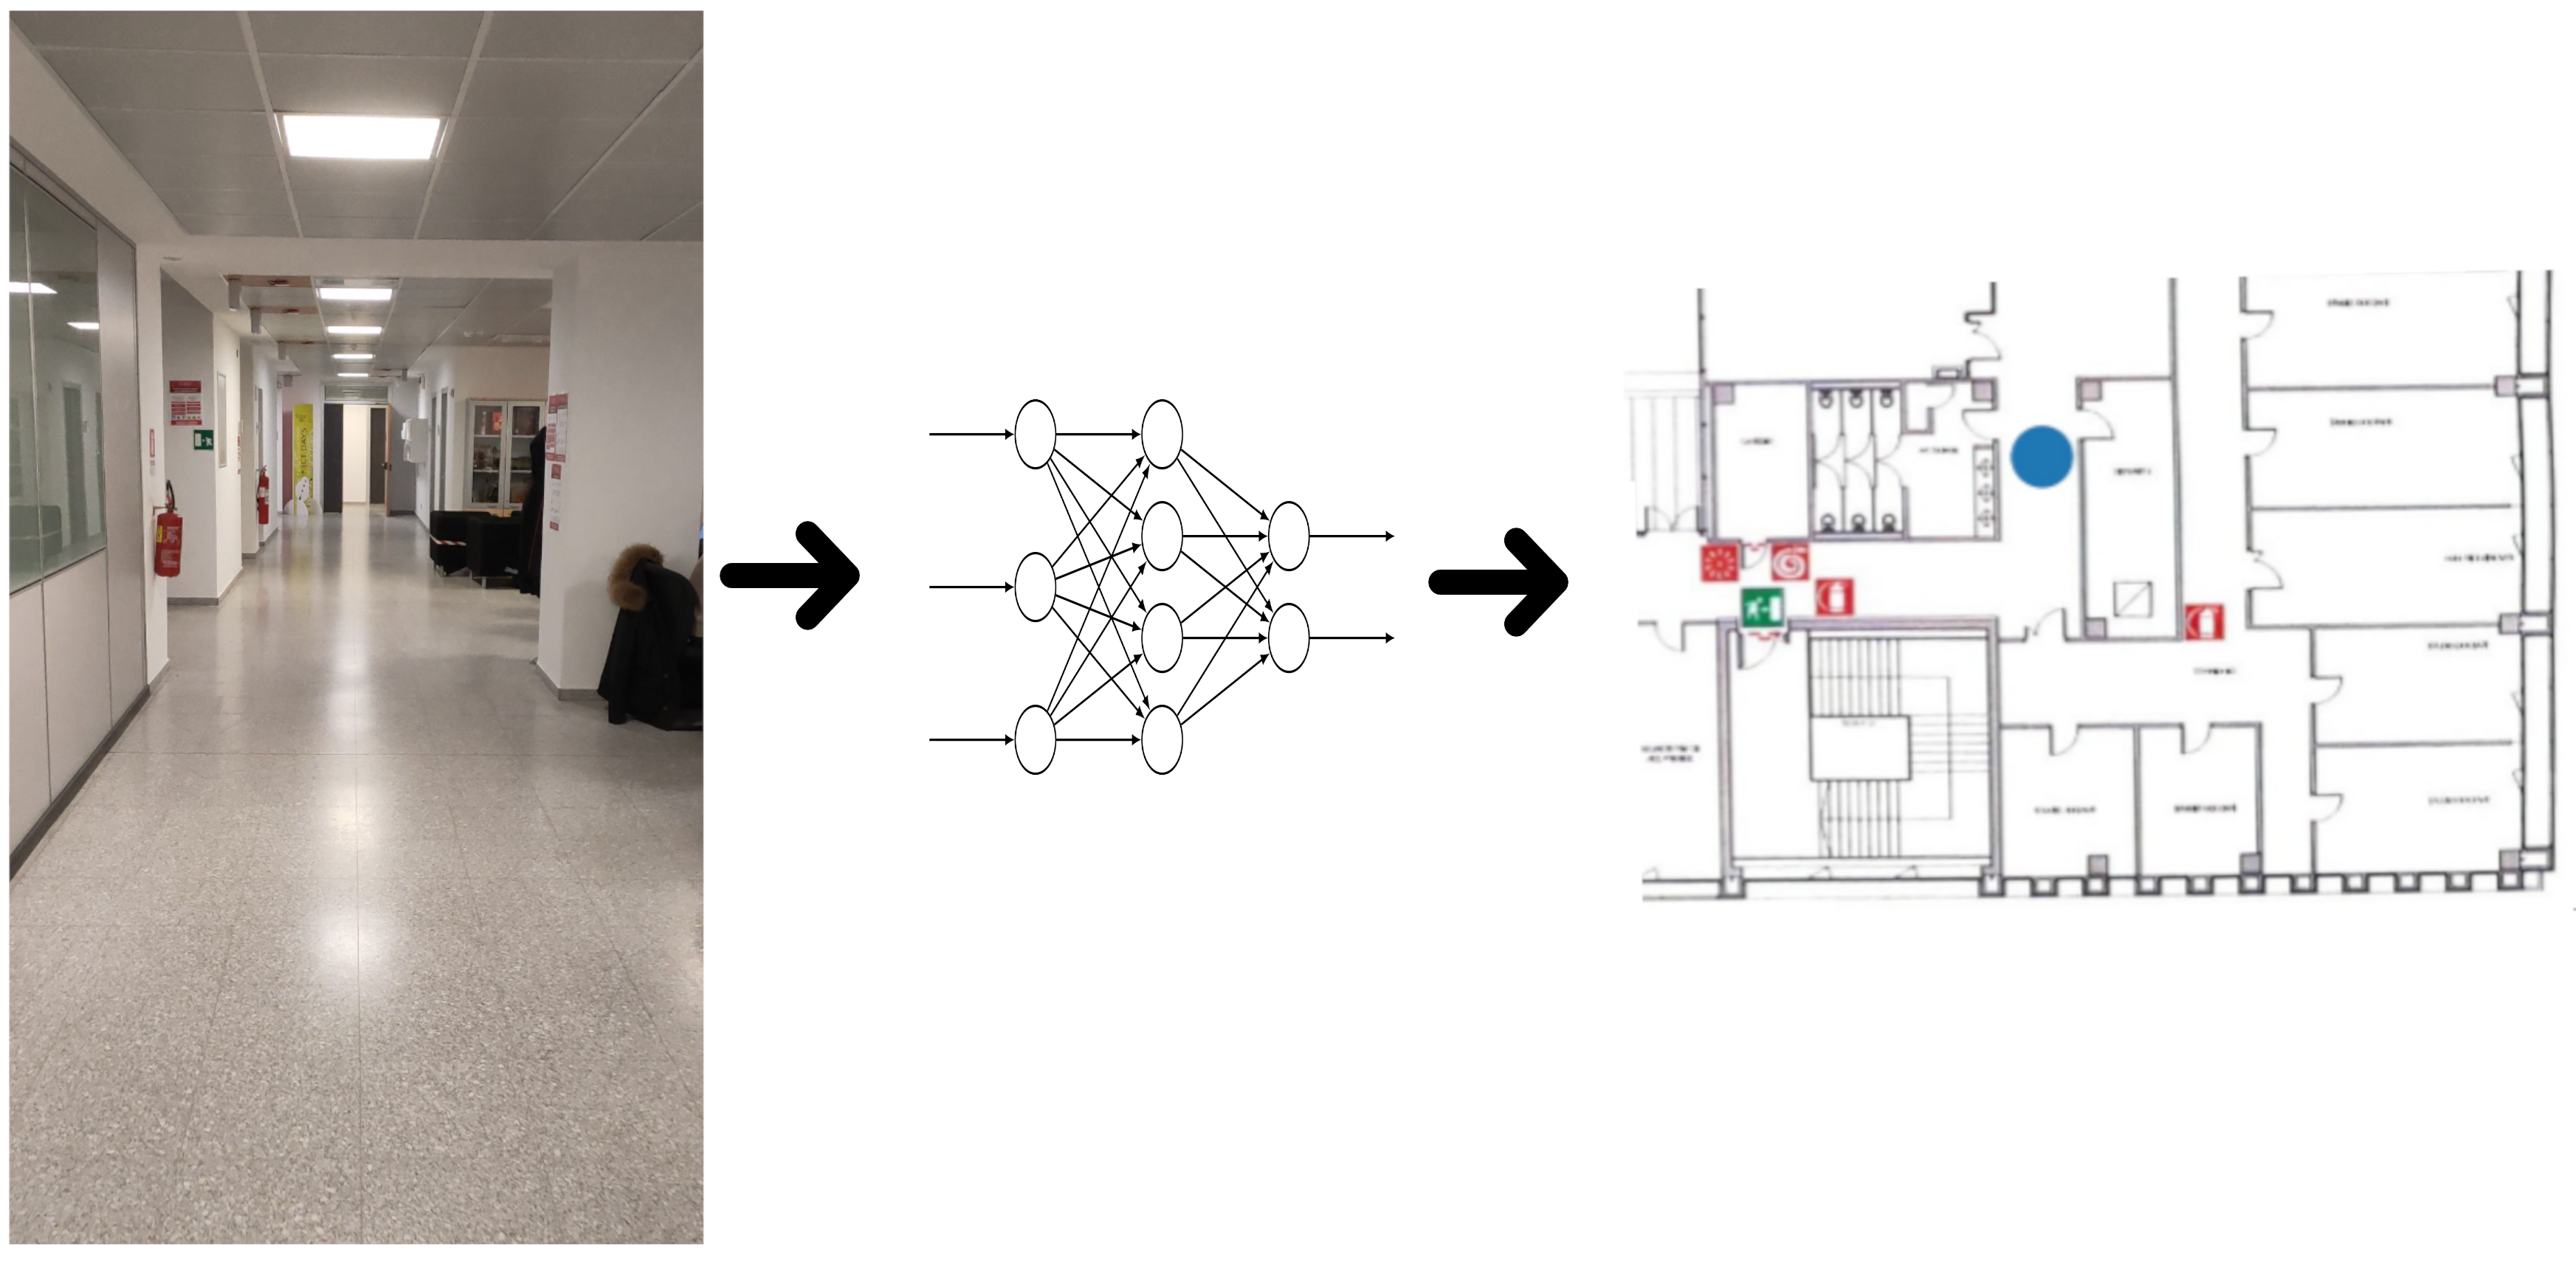
\includegraphics[width=0.9\textwidth]{../imgs/introduction_example.png}
            \caption{Camera pose estimation example.}
        \end{figure}

        \column{0.45\textwidth}
        The \textbf{camera pose estimation} $E$ is a task that, given an \textbf{image} $I_c$ acquired with a camera, processes it and returns a pair of \textbf{position} $x_c$ and \textbf{orientation} $q_c$.
    \[
        E(I_c) = (x_c, q_c)
    \]
    \end{columns}
\end{frame}

\section{Dataset}
% presentation of the 4 different attempts for dataset generation
\begin{frame}{Dataset generation tested approaches}
    Four different techniques have been tried during the project:
    \begin{itemize}
        \item \textbf{IMU sensors}: not enough accurate;
        \item \textbf{digital video}: not available in the university environment;
        \item \textbf{motion capture system}: not associable with a recorder video;
        \item \textbf{strcuture from motion}: usable in the context of this project
    \end{itemize}
\end{frame}
% COLMAP: introduction with some examples
\begin{frame}{COLMAP}
    COLMAP is \textbf{structure from motion} tool that allows ot reconstruct 3D representations of an environment using images of it. (non so che immagine mettere qui)
\end{frame}
% Uni Povo2: some screens and stats
\begin{frame}{Povo 1 second floor dataset}
    \begin{columns}
        \column{0.45\textwidth}
        \begin{figure}
            \centering
            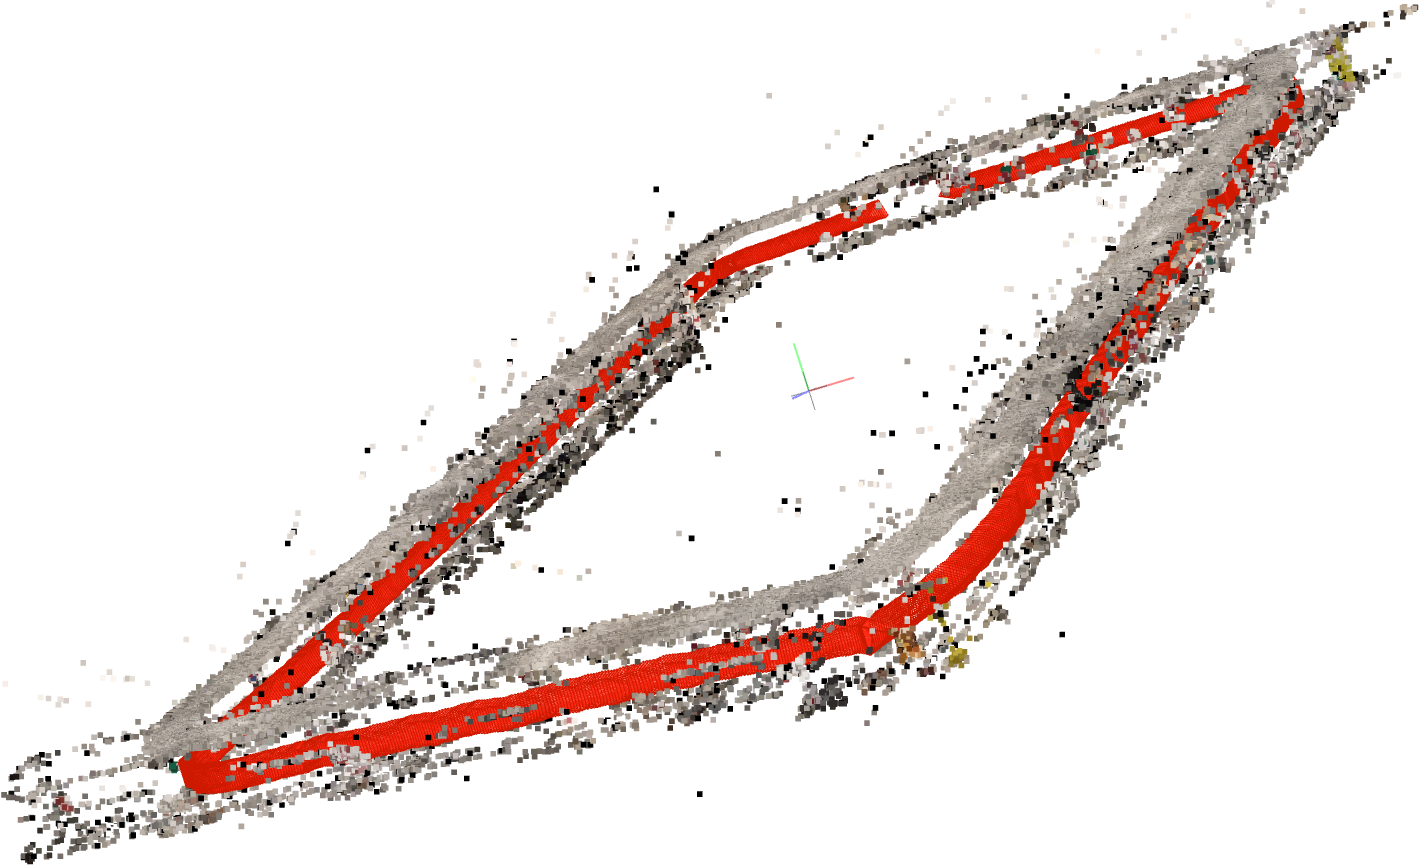
\includegraphics[width=0.9\textwidth]{../imgs/extracted_features_colmap.png}
            \caption{Trajectory and extracted features of Povo 2}
        \end{figure}

        \column{0.45\textwidth}
        After many attempts of environment reconstructions with COLMAP the final labeled dataset of \textbf{Povo 2 second floor} was created. \textbf{Red} lines is the \textbf{trajectory} and other points are \textbf{features}.
    \end{columns}
\end{frame}

% CRS alignment
\begin{frame}{Coordinate Reference System}
    \begin{columns}
        \column{0.45\textwidth}
        \begin{figure}
            \centering
            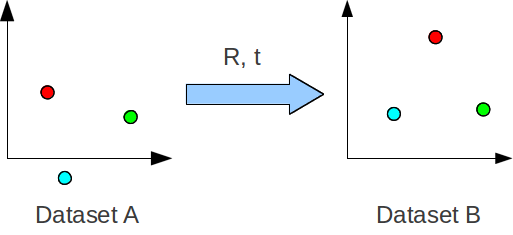
\includegraphics[width=0.9\textwidth]{../imgs/rigid_trasform.png}
            \caption{Rigid transform.}
        \end{figure}

        \column{0.45\textwidth}
        The \textbf{Coordinate Reference System} chosen by the reconstruction of COLMAP may not concide. It is required to apply some \textbf{transformations} to poses extracted from COLMAP model:
        \begin{enumerate}
            \item \textbf{scale};
            \item \textbf{translate};
            \item \textbf{rotate};
        \end{enumerate}
    \end{columns}
\end{frame}

\section{Models}
\subsection{MeNet}
\begin{frame}{The MeNet Model for Relative Pose Estimation}
    \begin{columns}
        \column{0.45\textwidth}
        \begin{figure}
            \centering
            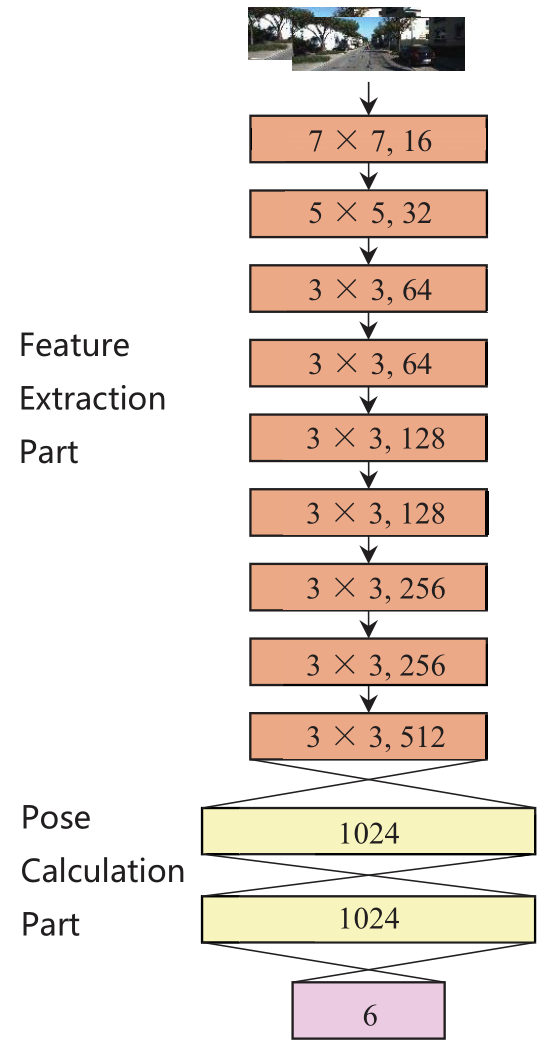
\includegraphics[width=0.9\textwidth]{../imgs/menet_structure.png}
            \caption{MeNet model architecture.}
        \end{figure}

        \column{0.45\textwidth}
        The \textbf{MeNet} model is targeted for \textbf{relative pose estimation}.
        The input of the network consists in a stack of two images: the goal is to estimate the relative pose of the second image with respect to the first one.
    \end{columns}
\end{frame}
\subsection{PoseNet}
\begin{frame}{The PoseNet Model for Absolute Pose Estimation}
    \begin{columns}
        \column{0.45\textwidth}
        \begin{figure}
            \centering
            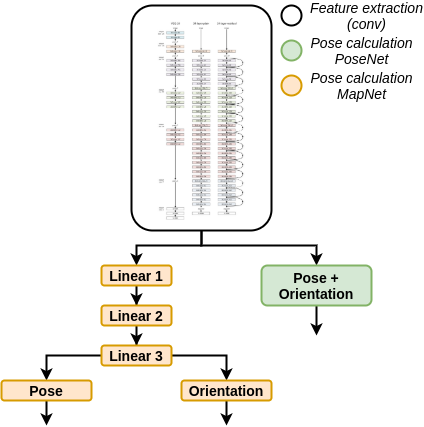
\includegraphics[width=0.9\textwidth]{../imgs/mapnet_posenet_structure.png}
            \caption{PoseNet model architecture.}
        \end{figure}

        \column{0.45\textwidth}
        The \textbf{PoseNet} model for absolute pose estimation is made up by two components:
        \begin{itemize}
            \item feature extraction through a sequence of convolutional layers (\emph{backend});
            \item pose regression on the extracted features using linear layers.
        \end{itemize}
    \end{columns}
\end{frame}
% PoseNet loss. General loss with h function (see MapNet loss in the report) with loss table and plot
\subsection{PoseNet losses}
\begin{frame}{The PoseNet losses}
    \begin{columns}
    \column{0.45\textwidth}
    \begin{figure}
        \centering
        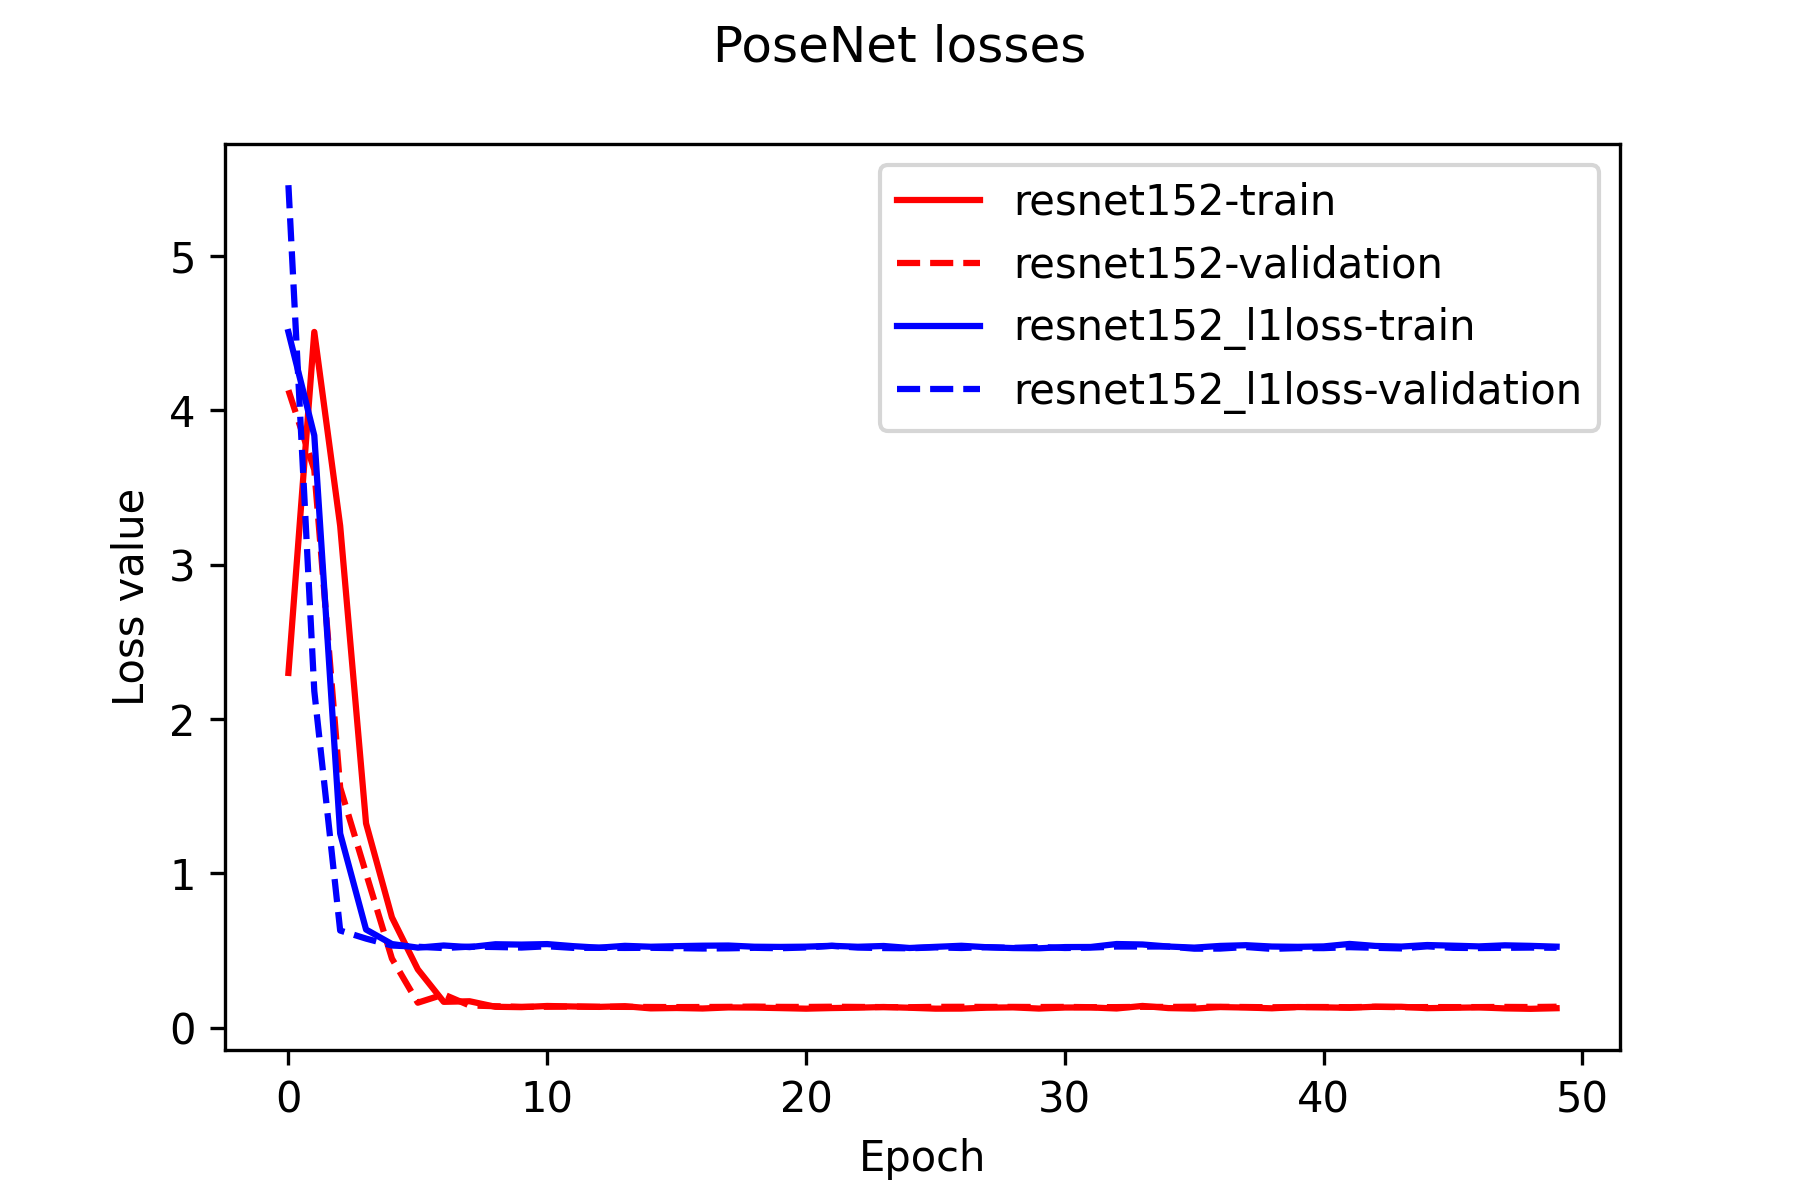
\includegraphics[width=0.9\textwidth]{../imgs/posenet_losses.png}
        \caption{PoseNet losses}
    \end{figure}
    % \begin{table}[htbp]
    %     \caption{PoseNet losses comparison}
    %     \begin{center}
    %         \begin{tabular}{lrr}
    %             \toprule
    %             Loss            & {Position Error} & {Rotation Error} \\
    %             \midrule
    %             SmoothedL1Loss  & \textbf{0.594}   & \textbf{0.139}   \\
    %             L1Loss          & 0.906            & 0.226            \\
    %             MSE             & NaN              & NaN              \\
    %             $\alpha \neq 1$ & NaN              & NaN              \\
    %             \bottomrule
    %         \end{tabular}
    %         \label{tab:posenet-losses}
    %     \end{center}
    % \end{table}

    \column{0.45\textwidth}
    Non ho idea di come far stare la tabella
    \begin{multline}
    Loss(w) = \frac{1}{N} \sum\limits_{i=1}^N h(P^i, \hat{P}^i) \\
    + \alpha h(Q^i, \hat{Q}^i)
    \end{multline}
    \end{columns}
\end{frame}
% PoseNet trajectory with 2000cm error
\subsection{PoseNet results}
\begin{frame}{The PoseNet losses}
    \begin{columns}
    \column{0.45\textwidth}
    \begin{figure}
        \centering
        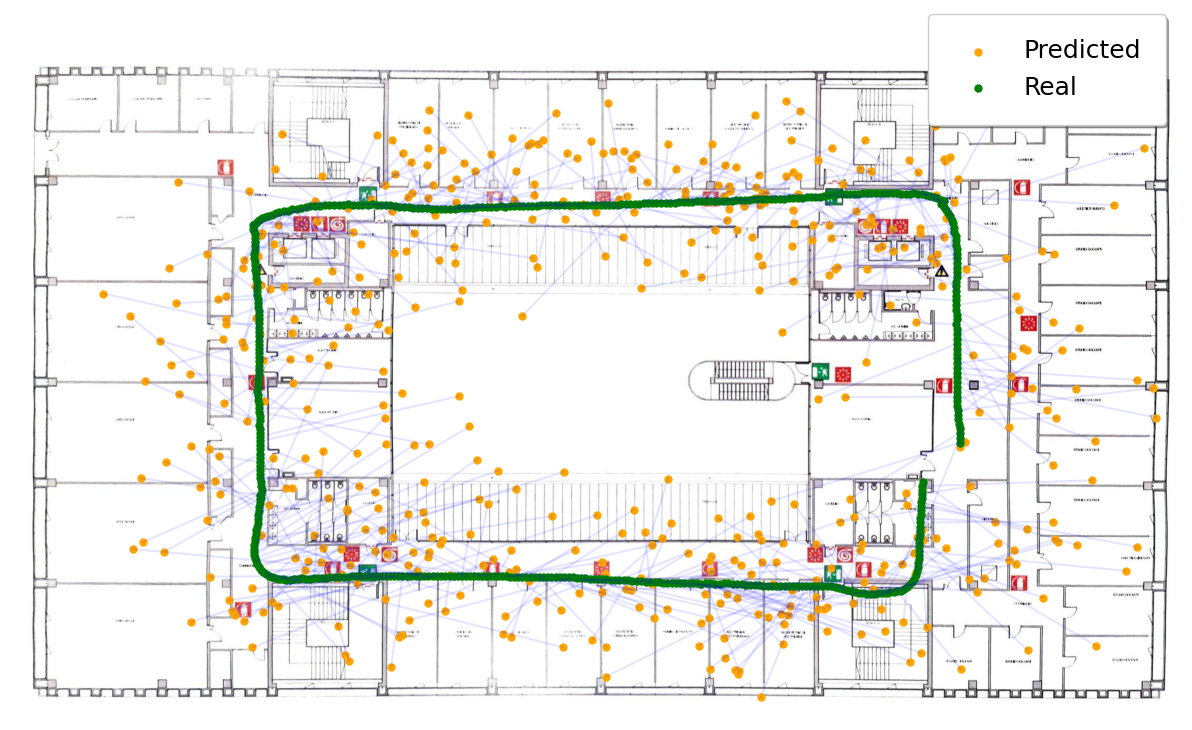
\includegraphics[width=0.9\textwidth]{../imgs/posenet_map.png}
        \caption{PoseNet predictions.}
    \end{figure}

    \column{0.45\textwidth}
    The predictions of the PoseNet (non so cosa scrivere)
    \end{columns}
\end{frame}

% Absolute pose estimation models with transfer learning + backend table on ImageNet
\subsection{MapNet}
\begin{frame}{The MapNet Model for Absolute Pose Estimation}
    \begin{columns}
        \column{0.45\textwidth}
        \begin{figure}
            \centering
            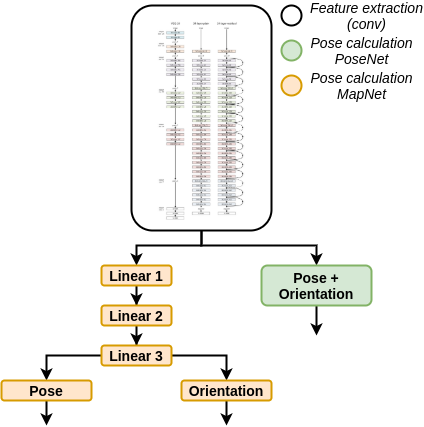
\includegraphics[width=0.9\textwidth]{../imgs/mapnet_posenet_structure.png}
            \caption{MapNet model architecture.}
        \end{figure}

        \column{0.45\textwidth}
        The \textbf{MapNet} model for absolute pose estimation represents an evolution of the PoseNet model with improvements:
        \begin{itemize}
            \item increase the number of final linear layers;
            \item penalize both absolute and relative errors in the loss.
        \end{itemize}
    \end{columns}
\end{frame}
% MapNet loss. General loss with h function with loss table and plot
\subsection{MapNet losses}
\begin{frame}{The MapNet losses}
    \begin{columns}
    \column{0.45\textwidth}
    \begin{figure}
        \centering
        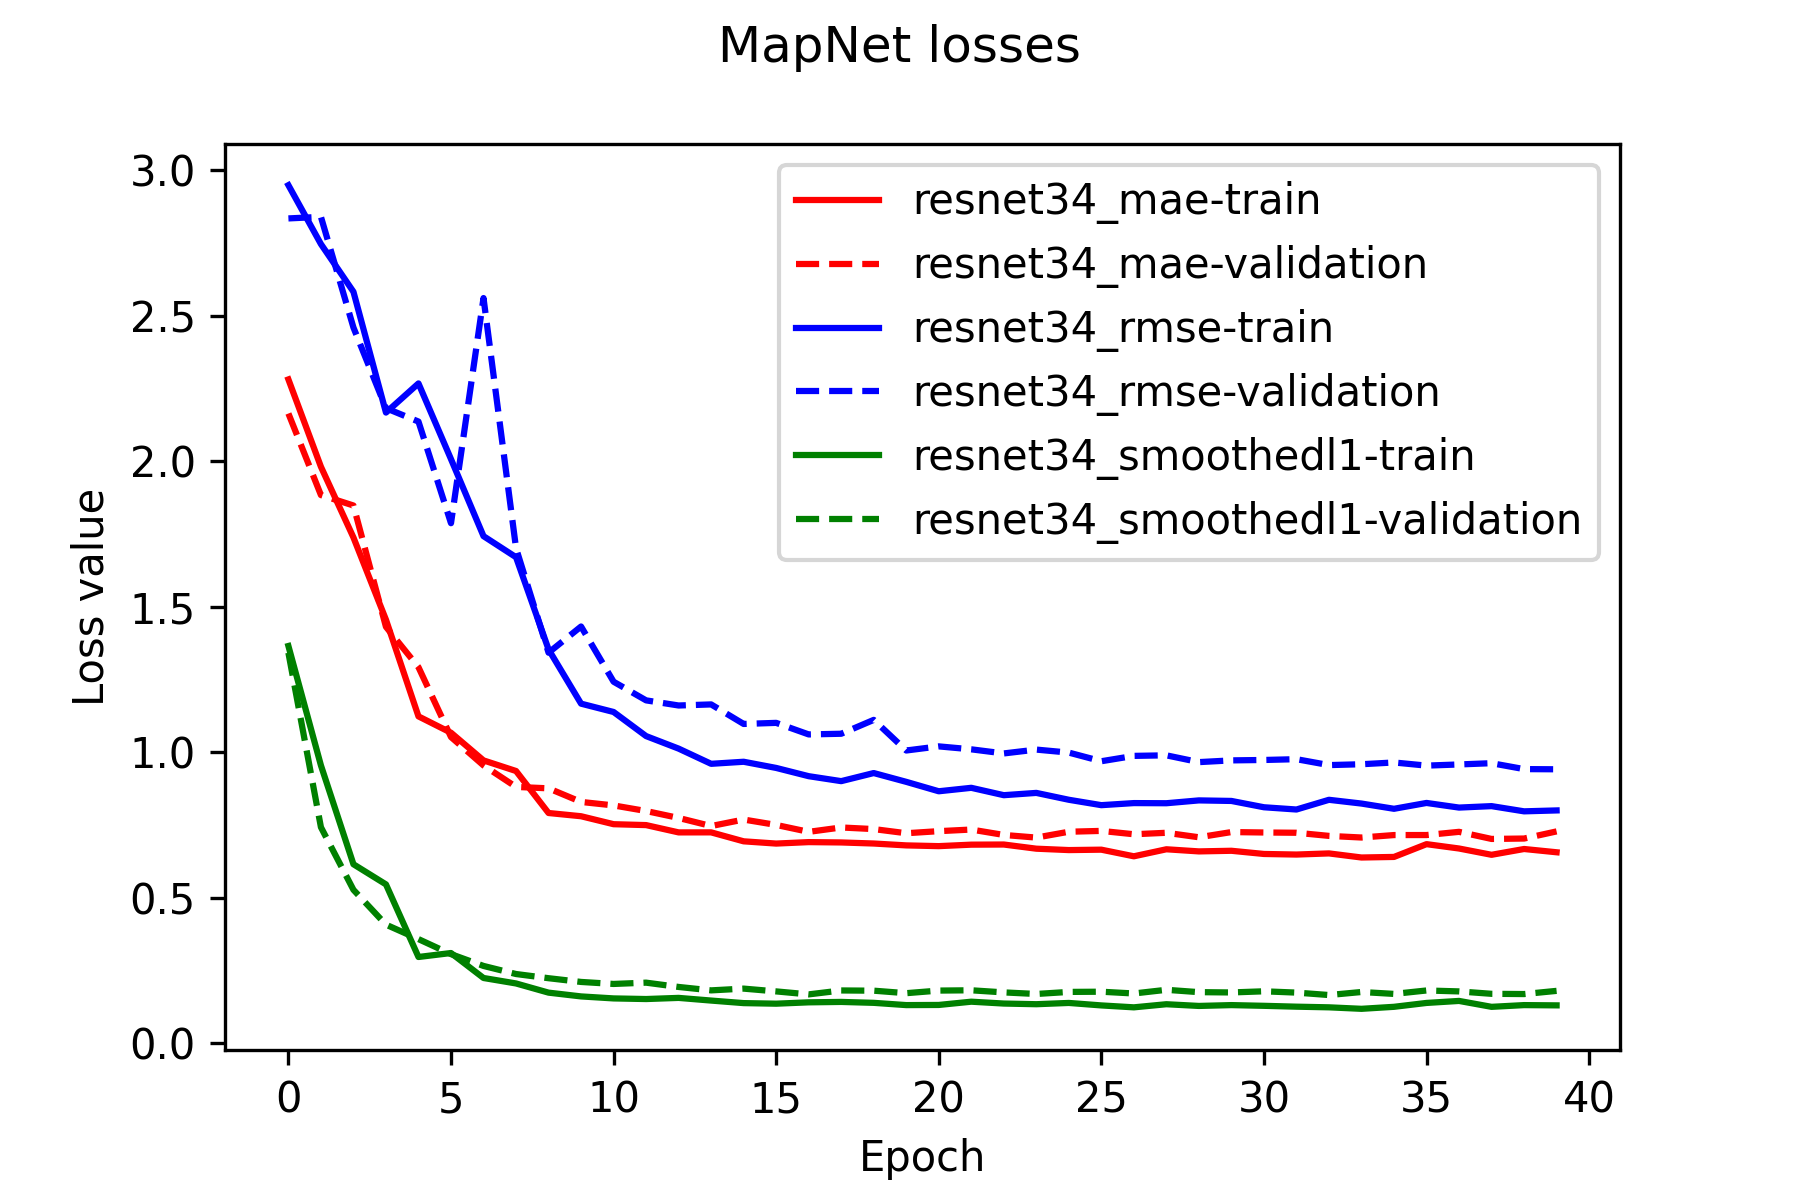
\includegraphics[width=0.9\textwidth]{../imgs/mapnet_losses.png}
        \caption{MapNet losses}
    \end{figure}
    % \begin{table}[htbp]
    %     \caption{Mapnet losses comparison}
    %     \begin{center}
    %         \begin{tabular}{lrr}
    %             \toprule
    %             Loss            & {Position Error} & {Rotation Error} \\
    %             \midrule
    %             L1Loss          & 0.227            & 0.042            \\
    %             SmoothedL1Loss  & 0.187            & 0.076            \\
    %             RMSE            & \textbf{0.187}   & \textbf{0.038}   \\
    %             \bottomrule
    %         \end{tabular}
    %         \label{tab:mapnet-losses}
    %     \end{center}
    % \end{table}
    %
    \column{0.45\textwidth}
    Non ho idea di come far stare la tabella
    \begin{multline}
    L_\mathcal{D}(\Theta) = \sum\limits_{i=1}^{|\mathcal{D}|} h([\hat{P}^i \hat{Q}^i], [P^i Q^i]) \\
    + \alpha\sum\limits_{i,j=1, i\neq j}^{|\mathcal{D}|} h([\hat{P}^{ij} \hat{Q}^{ij}], [P^{ij} Q^{ij}])
    \end{multline}
    \end{columns}
\end{frame}
% MapNet trajectory with 153cm error
\subsection{MapNet results}
\begin{frame}{The MapNet losses}
    \begin{columns}
    \column{0.45\textwidth}
    \begin{figure}
        \centering
        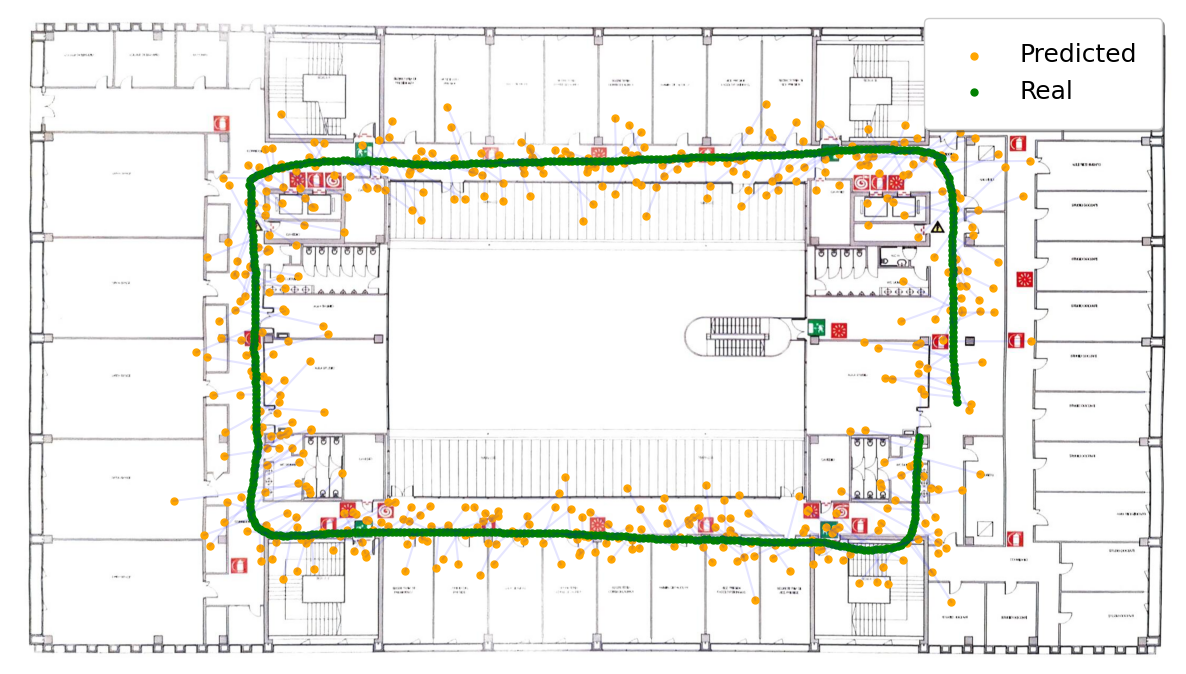
\includegraphics[width=0.9\textwidth]{../imgs/mapnet_map.png}
        \caption{MapNet predictions.}
    \end{figure}

    \column{0.45\textwidth}
    The predictions of the MapNet (non so cosa scrivere)
    \end{columns}
\end{frame}
% Post-processing: new trajectory with new error
\begin{frame}{Post-processing algorithm}
    \begin{columns}
        \column{0.45\textwidth}
        \begin{figure}
            \centering
            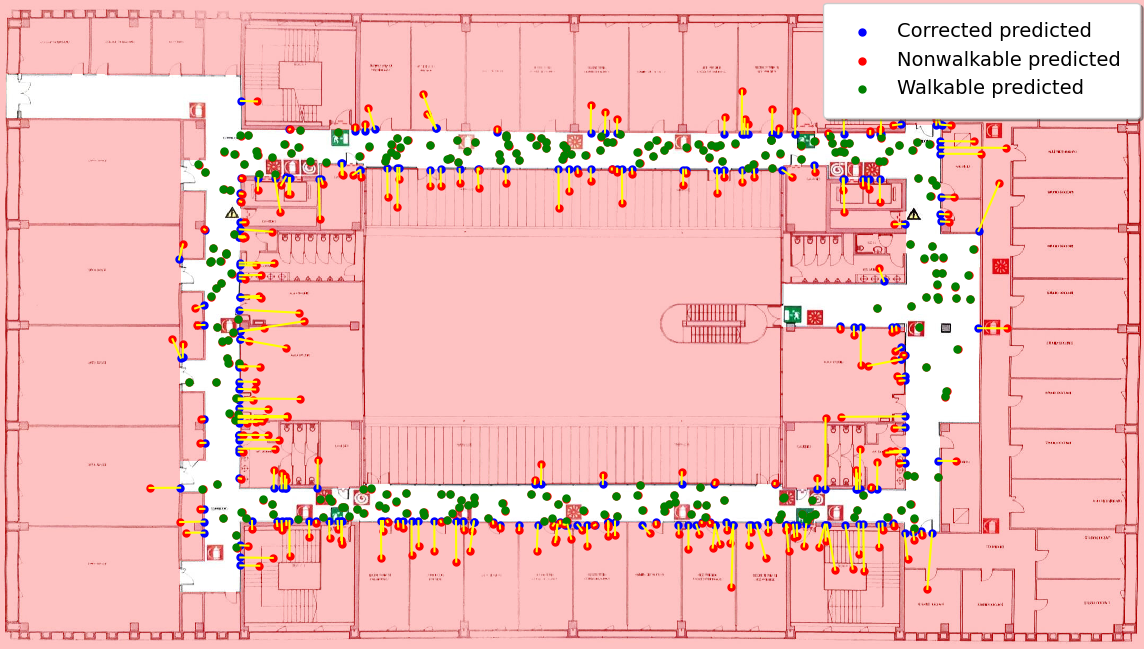
\includegraphics[width=0.9\textwidth]{../imgs/walkable_postprocess.png}
            \caption{Prediction map after post-processing procedure.}
        \end{figure}

        \column{0.45\textwidth}
        Post-process technique base on Euclidean distance in order to fix non walkable predictions.
    \end{columns}
\end{frame}
% Dashboard screen
\begin{frame}{The MapNet Model for Absolute Pose Estimation}
    \begin{columns}
        \column{0.45\textwidth}
        \begin{figure}
            \centering
            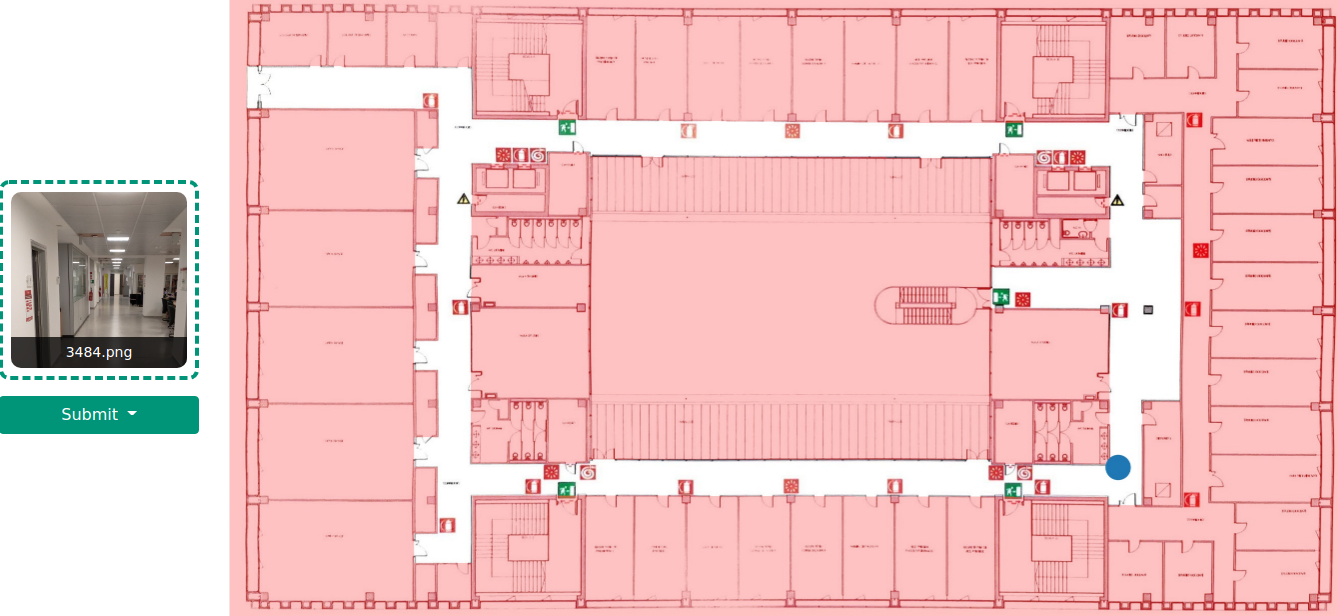
\includegraphics[width=0.9\textwidth]{../imgs/dashboard.png}
            \caption{FastAPI dashboard that serves the model.}
        \end{figure}

        \column{0.45\textwidth}
        TODO
    \end{columns}
\end{frame}

\section{Conclusions}
\begin{frame}{Conclusions}
    To summarize, the final results presented in this work are:
    \begin{itemize}
        \item the exploration of multiple dataset generation techniques;
        \item the COLMAP reconstruction of Povo 1 second floor;
        \item the development of relative and absolute pose estimation models;
        \item the fine-tuning of absolute pose estimation models;
        \item the post-processing of the model outputs;
        \item the model deployment using a FastAPI web-server. 
    \end{itemize}
\end{frame}

% \begin{frame}{Block examples}
%     \begin{block}{Observation 1}
%         Simmons Hall is composed of metal and concrete.
%     \end{block}
%     \begin{exampleblock}{Observation 2}
%         Simmons Hall is composed of metal and concrete.
%     \end{exampleblock}
%     \begin{textbfblock}{Conclusion}
%         Simmons Hall $\not=$ Simmons Dormitory.
%     \end{textbfblock}
% \end{frame}
\end{document}
